\documentclass[11pt,a4paper]{report}
\usepackage[portuges]{babel}
\usepackage[utf8]{inputenc} % define o encoding usado texto fonte (input)--usual "utf8" ou "latin1
\usepackage{graphicx} %permite incluir graficos, tabelas, figuras
\usepackage{subcaption}
\usepackage[title]{appendix}
\usepackage{listings}
\usepackage{color}
\usepackage{multicol}
\usepackage{indentfirst}
\usepackage{hyperref}
\usepackage{amsmath}
\usepackage{amssymb}
\usepackage{float}
\usepackage{enumerate}
\usepackage[shortlabels]{enumitem}
\usepackage[T1]{fontenc}
\usepackage{hyperref}



\definecolor{mygreen}{rgb}{0,0.6,0}
\definecolor{mygray}{rgb}{0.5,0.5,0.5}
\definecolor{mymauve}{rgb}{0.58,0,0.82}

\hypersetup{
    colorlinks=true,
    linkcolor=blue,
    urlcolor=black,
    }
    
    
    
\usepackage{bera}% optional: just to have a nice mono-spaced font

\definecolor{eclipseStrings}{RGB}{42,0.0,255}
\definecolor{eclipseKeywords}{RGB}{127,0,85}
    

\lstset{ %
  backgroundcolor=\color{white},   % choose the background color
  basicstyle=\footnotesize,        % size of fonts used for the code
  breaklines=true,                 % automatic line breaking only at whitespace
  captionpos=b,                    % sets the caption-position to bottom
  commentstyle=\color{mygreen},    % comment style
  escapeinside={\%*}{*)},          % if you want to add LaTeX within your code
  keywordstyle=\color{blue},       % keyword style
  stringstyle=\color{mymauve},     % string literal style
}



\title{POO - Trabalho Prático\\
	\large Grupo nº5}

\author{Simão Pedro Batista Caridade Quintela \\ (A97444) 
             \and Pedro Alexandre Silva Gomes \\ (A91647)
             \and Gonçalo da Silva \\ (A95696)
       } %autores do documento
       
\date{\today} %data

\begin{document}
	\begin{minipage}{0.9\linewidth}
        \centering
		
\includegraphics[width=0.4\textwidth]{um.jpg}\par\vspace{1 cm}
		\href{https://www.uminho.pt/PT}
		{\scshape\LARGE Universidade do Minho} \par
		\vspace{0.6cm}
		\href{https://lcc.di.uminho.pt}
		{\scshape\Large Licenciatura em Ciências da Computação} \par
		\maketitle
		\begin{figure}[H]
			
\includegraphics[width=0.345\linewidth]{placaUni.jpeg}
			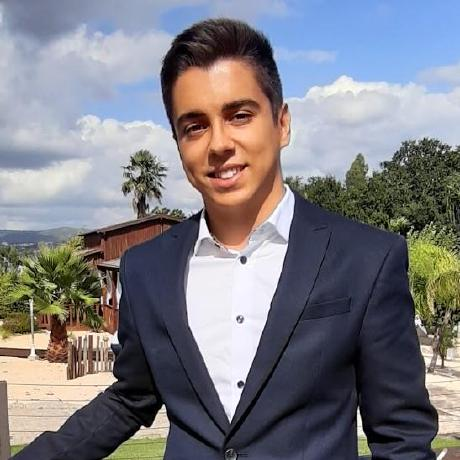
\includegraphics[width=0.32\linewidth]{pedro.jpg}
    		
\includegraphics[width=0.32\linewidth]{goncalo.png}
		\end{figure}
	\end{minipage}
	
	\tableofcontents
	
	\pagebreak
	
	\chapter{Introdução}
%	
	Este relatório descreve o desenvolvimento do projeto prático da Unidade Currícular de Programação Orientada aos Objetos, inserida no 2ºano da Licenciatura em Ciências da Computação da Universidade do Minho.
	
	Este trabalho consistia no desenvolver de um sistema que monitorize e registe a informação sobre o consumo
energético das habitações de uma comunidade. Em cada casa existe um conjunto muito alargado de dispositivos que são todos controlados a partir deste programa, os \textit{SmartDevice}. Para que a realização do referido fosse possível, utilizamos os conhecimentos da linguagem \textit{Java}, adquiridos ao longo do semestre.  
	
	\pagebreak
	
	\chapter{Estrututa do projeto}

O nosso projeto segue o modelo de estrutura \textbf{\textit{Model View Controller} (MVC)}, que consite na organização deste em três camadas:
	\begin{itemize}
		\item A camada de dados \textbf{(o modelo)} é composta pelas classes \textit{CasaInteligente, SmartDevice, SmartBulb, SmartSpeaker, SmartCamera, Comercializador, Fatura, Comunidade, Tuple, SaveProgramText, Parser, SimulParser}.
		\item A camada de interação com o utilizador \textbf{(a vista, ou apresentação)} é composta unicamente pela classe \textit{View}.
		\item A camada de controlo do fluxo do programa\textbf{ (o controlador)} é composta pela classe \textit{Controller}.
	\end{itemize}
        Em todo o projeto respeitamos a ideia de encapsulamento, como pedido, utilizando a estratégia de \textbf{agregação}.


\pagebreak

	\chapter{Classes}
	
	Estas são as classes que constituem o nosso programa:
	
    \section{App}
    \begin{lstlisting}[language=java,firstnumber=1]
    static Scanner scan = new Scanner(System.in);
    static Controller controller = new Controller(comunidade);
    \end{lstlisting}
    
    Esta classe contém a \textit{main} do programa na qual este é inicializado.
    Nesta mesma classe são inicializados o \textit{ Controller}, a \textit{View} e o \textit{ Scanner}, sendo a \textit{View} inicializada com os parâmetros \textit{ Controller} e \textit{ Scanner}.
    
    \section{Comunidade}
	\begin{lstlisting}[language=java,firstnumber=1]
    private String nomeDaComunidade;
    private Map<String, CasaInteligente> casas; // proprietario -> Casa
    private Map<String, Comercializador> mercado; // fornecedor -> Comercializador
    \end{lstlisting}
    
    Esta classe tem como propósito guardar todas as casas criadas, bem como comercializadores e o nome dado à própria comunidade. Para isso, utilizamos dois \textbf{Maps} sendo que o primeiro associa o proprietário ao objeto casa e o segundo associa o fornecedor ao objeto fornecedor.  
    
	\section{CasaInteligente}
	
	O \textbf{package CasaInteligente} contém as classes \textit{CasaInteligente}, todos os tipos de \textit{SmartDevices} incluindo a classe abstrata \textit{SmartDevice} e todas as classes de Test associadas a estas.
	
	\subsection{CasaInteligente}
	\begin{lstlisting}[language=java,firstnumber=1]
    private String proprietario;
    private int NIF;
    private String fornecedor;
    private Map<String, SmartDevice> devices; // identificador -> SmartDevice
    private Map<String, List<String>> locations; // Espaço -> Lista codigo dos devices
    private List<Fatura> faturas; // lista de faturas que foram geradas e associadas à casa
    \end{lstlisting}
    
    Esta classe tem várias variáveis de intância com informação acerca da casa e do seu proprietário. Em termos de estruturas de dados, utilizamos um \textbf{Map} para guardar os \textit{SmartDevices} da casa em que a\textbf{ key} é o\textbf{ ID} do device do tipo\textbf{ String} e o correspondente \textbf{value} é o objeto\textit{ SmartDevice} associado. Utilizamos também outro \textbf{Map} que, a cada divisão, associa uma lista de \textbf{IDs} de \textit{SmartDevices}, que nela estão contidos, sendo que as \textbf{keys} são \textbf{Strings} a representar o nome da divisão e os \textbf{values }são do tipo \textbf{List<String>} no qual guardamos os \textbf{IDs} dos \textit{SmartDevices} presentes na divisão. Por fim, temos uma estrutura \textbf{List<Fatura>} para guardar na casa todas as faturas emitidas cujo o destinatário é a própria casa. 
    
	\subsection{CasaInteligenteTest}
	
	Esta classe contém alguns testes que fomos utilizando durante o desenvolver do projeto.
	
	\subsection{SmartDevices}
	
	Este \textbf{package} contém todas as classes correspondentes aos SmartDevices e respetivos testes. 
	
        \begin{itemize}
        \item SmartDevice
        \begin{lstlisting}[language=java,firstnumber=1]
    private String id;
    private boolean on;
    private LocalDate time;
    private float consumption;
    private float consumptionPerDay;
    private int custoInstalacao;
    \end{lstlisting}
    
    Esta é uma classe que tem por objetivo a repretentação dos 3 tipos de \textit{SmartDevices(SmartBulb, SmartCamera e SmartSpeaker)}. Decidimos que esta seria uma classe abstrata, devido ao facto de, os diferentes tipos de\textit{ SmartDevices} terem muita informação em comum \textbf{(ID, Estado, ConsumoEnergetico, ...)}, ou seja, a nossa intenção foi agrupar todas as características numa classe genérica, em que os diferente tipos de \textit{SmartDevices} a extendem e a variação de informação entre \textit{SmartDevices} é feita na própria classe correspondente do \textit{SmartDevice}.  
    
        \item SmartDeviceTest
        \item SmartBulb
        \begin{lstlisting}[language=java,firstnumber=1]
    private static final int WARM = 80;
    private static final int NEUTRAL = 60;
    private static final int COLD = 40;
    private int tone;
    private int dimensions;
    \end{lstlisting}
    
    Esta classe contém todas as informações relevantes quanto a\textit{ SmartBulb}(tonalidade em que está ligada, dimensões) e possui métodos que contam o consumo energético num dado período de tempo, bem como métodos de\textbf{ turnOn} e \textbf{turnOff}.
    
        \item SmartBulbTest
        \item SmartSpeaker
        \begin{lstlisting}[language=java,firstnumber=1]
    private static final int MAX = 100; //volume maximo
    private int volume;
    private String channel;
    private String brand;
    \end{lstlisting}
    
    Esta classe contém todas as informações relevantes quanto a\textit{ SmartSpeaker}(volume, marca e canal em que está ligado) e possui métodos que contam o consumo energético num dado período de tempo, bem como métodos de\textbf{ turnOn}, \textbf{turnOff}, \textbf{VolumeUp} e \textbf{VolumeDown}.
    
        \item SmartCamera
        \begin{lstlisting}[language=java,firstnumber=1]
    private int xRes;
    private int yRes;
    private int fileSize;
    private float custoInstalacao;
    \end{lstlisting}
    
    Esta classe contém todas as informações relevantes quanto a\textit{ SmartCamera}(resolução e tamanho de ficheiro) e possui métodos que contam o consumo energético num dado período de tempo, bem como métodos de\textbf{ turnOn}, \textbf{turnOff}.
    
        \end{itemize}
        
	\section{ComercializadoresEnergia}
	
	Neste\textbf{ package} estão todas as classes relacionadas com fornecedores de energia.
	
	\subsection{Comercializador}
	\begin{lstlisting}[language=java,firstnumber=1]
    private String nomeEmpresa;
    private int numeroDispositivos;
    private int valorBase;
    private int imposto;
    private Map<String, List<Fatura>> faturas;  // Proprietário -> Lista de Faturas
    \end{lstlisting}
    
    Esta classe representa um Comercializador de Energia e contém informação sobre o mesmo como, por exemplo, \textbf{nome da empresa, valor base, imposto, etc...} .
    Quanto à fórmula escolhida para cada fornecedor, tentamos dar uma certa liberdade ao fornecedor de poder escolher um número dispositivos que, quando ultrapassado, a cobrança seja diferente. A fórmula escolhida foi:
    
    \begin{lstlisting}[language=java,firstnumber=1]
    if(numeroDispositivosCasa > numeroDispositivos(var. de instancia))
        consumo = consumoDoDispositivo / 1500 * (imposto / 100) * 0.9
    else
        consumo = consumoDoDispositivo / 1500 * (imposto / 100) * 0.75
    \end{lstlisting}
    
    Quanto a estruturas de dados, utilizamos um \textbf{Map} para guardar todas as faturas emitidas pelo comercializador em questão, sendo que as \textbf{keys} são o nome do proprietário da casa e os values são a lista de faturas emitidas para a mesma do tipo \textbf{List<Fatura>}.
	
	\subsection{Fatura}
	\begin{lstlisting}[language=java,firstnumber=1]
    private int codigo;
    private int nif;
    LocalDate dataEmissao;
    private float total;
    private String empresa;
    private String cliente;
    \end{lstlisting}
    
    A classe \textit{Fatura} representa um objeto fatura que é utilizado para registar o consumo de uma casa num dado período de tempo. Para isso, utilizamos variáveis como, \textbf{cliente, empresa, dataEmissao, etc...} .
    
    \section{ConsumeComparator}
    
    Esta classe é usada para comparar consumos.
    
    \section{View}
    \begin{lstlisting}[language=java,firstnumber=1]
    private Controller controller;
    private Scanner scan;
    \end{lstlisting}
    
    A \textit{View} é a classe como a qual se faz a interação com o utilizador. Para isso, solicita operações ao Controller que são respondidas com sucesso. 
	
	\section{Controller}
	\begin{lstlisting}[language=java,firstnumber=1]
    private Comunidade comunidade;
    private int idFatura;
    private LocalDate timeNow;
    \end{lstlisting}
    
    A classe\textit{ Controller} satisfaz os pedidos da \textit{View} e, para isso, utiliza 3 variáveis de instância \textbf{(comunidade, idFatura e timeNow)}. A variável \textbf{comunidade} guarda a comunidade inicializada à criação do \textit{Controller}, a \textbf{idFatura} guarda o número de faturas criadas e a variável \textbf{timeNow} guarda o tempo atual em que está a correr o programa.
	
    \section{Parser}
    
    A classe\textit{ Parser} lê um ficheiro de texto com informações acerca da comunidade e gera todos os objetos resultantes disso.\\
    Fornecedor:<NomeFornecedor>, <NumeroDispositivos>\\
    Casa:<NomeProprietario>,<NifProprietario>,<NomeFornecedor>\\
    DivisaoEDevices:<Divisao>,<Devices>\\
    SmartCamera:<Resolucao>,<Tamanho>,<Consumo>\\
    SmartSpeaker:<Volume>,<CanalRadio>,<Marca>,<Consumo>

    \section{SaveProgramText}
    
    Esta classe tem como objetivo gravar o programa num ficheiro de texto.
    
    \section{SimulParser}
    
    A classe \textit{SimulParser} é utilizada para ler o ficheiro de configuração de uma simulação.\\
    Demos a possibilidade do utilizador realizar 6 ações:
    \begin{enumerate}
    \item Turn On (turnOn)
    \item Turn Off (turnOff)
    \item Mudar de fornecedor (mudar)
    \item Mudar número de dispositivos num fornecedor (mudarNumDisp)
    \item Mudar localização de um dispositivo (novaLoc)
    \item Remover um dispositivo (remover)
    \end{enumerate}
    Foram usadas as seguintes convenções:\\
    data,proprietario,idDispositivo,turnOn\\
    data,proprietario,idDispositivo,turnOff\\
    data,proprietario,fornecedor,mudar\\
    data,fornecedor,numDispositivos,mudarNumDisp\\
    data,proprietario,idDispositivo,novaLoc,localizacao\\
    data,proprietario,idDispositivo,remover
    
    \section{Tuple}
    \begin{lstlisting}[language=java,firstnumber=1]
    private String p1;
    private float p2;
    \end{lstlisting}
    
    A classe \textit{Tuple} foi criada para responder à necessidade de retornar mais do que um parâmetro ao desenvolver as estatísticas do programa, sendo as variáveis de instância \textbf{p1} e \textbf{p2} o primeiro e segundo elemento do tuplo, respetivamente.
    
	\pagebreak
	
	\section{Diagrama de classes do \textit{blueJ}}
	
	\begin{figure}[H]
			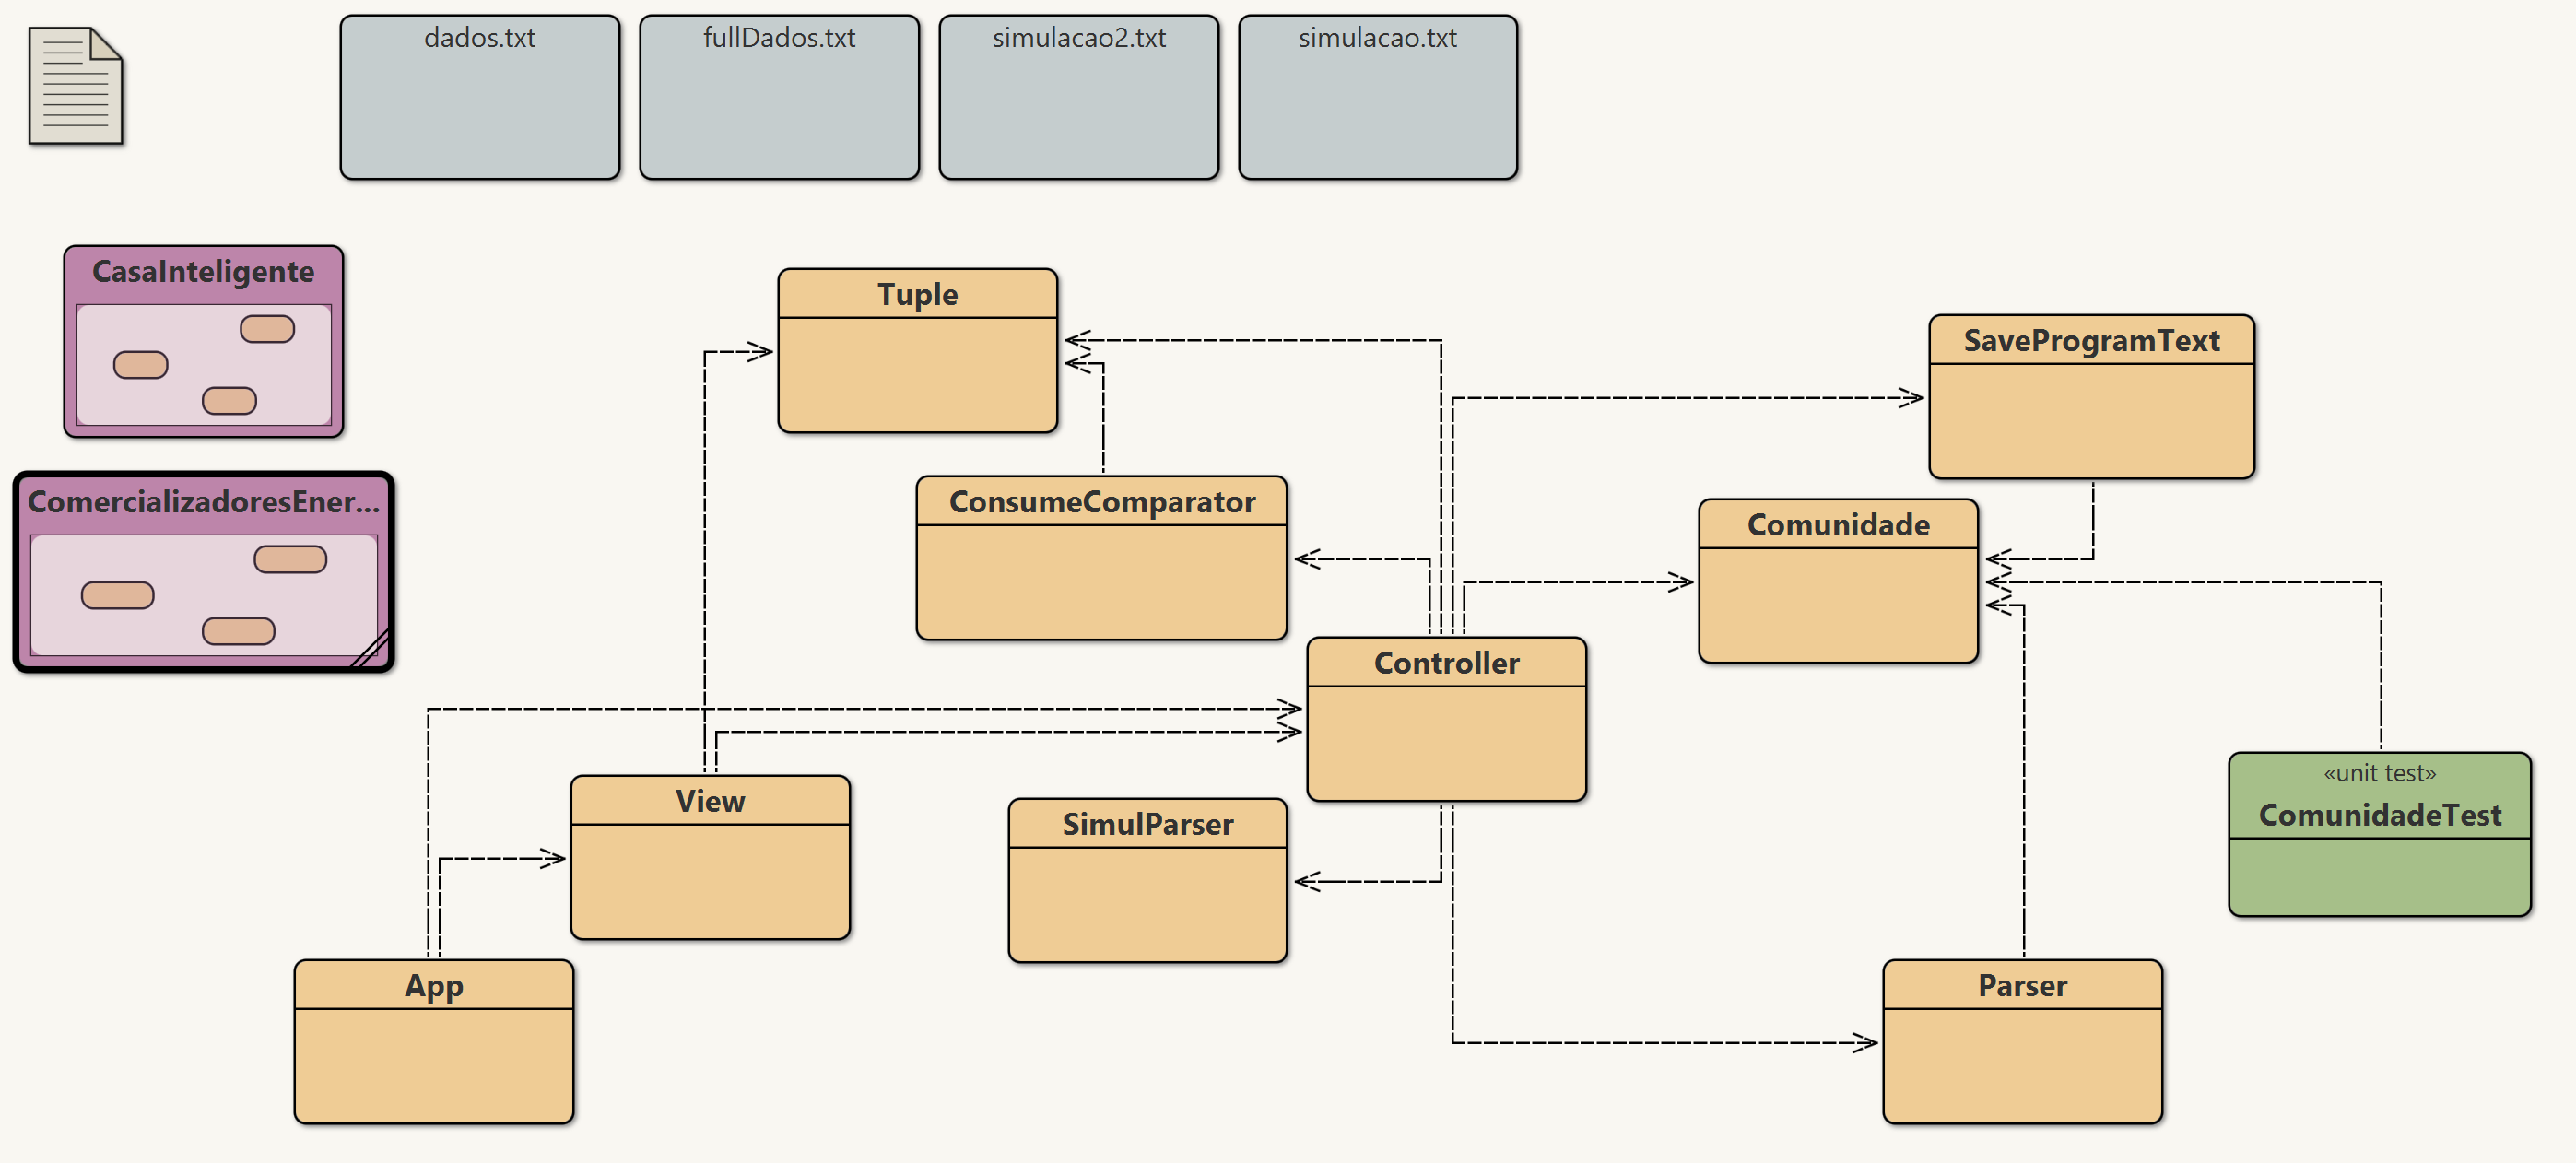
\includegraphics[scale=0.16]{diagrama1.png}
	\end{figure}
	
\begin{enumerate}
    \item Diagrama principal com as super classes, interfaces de simulação e ficheiros .txt
    \vspace{13mm} %5mm vertical space

	\begin{figure}[H]
			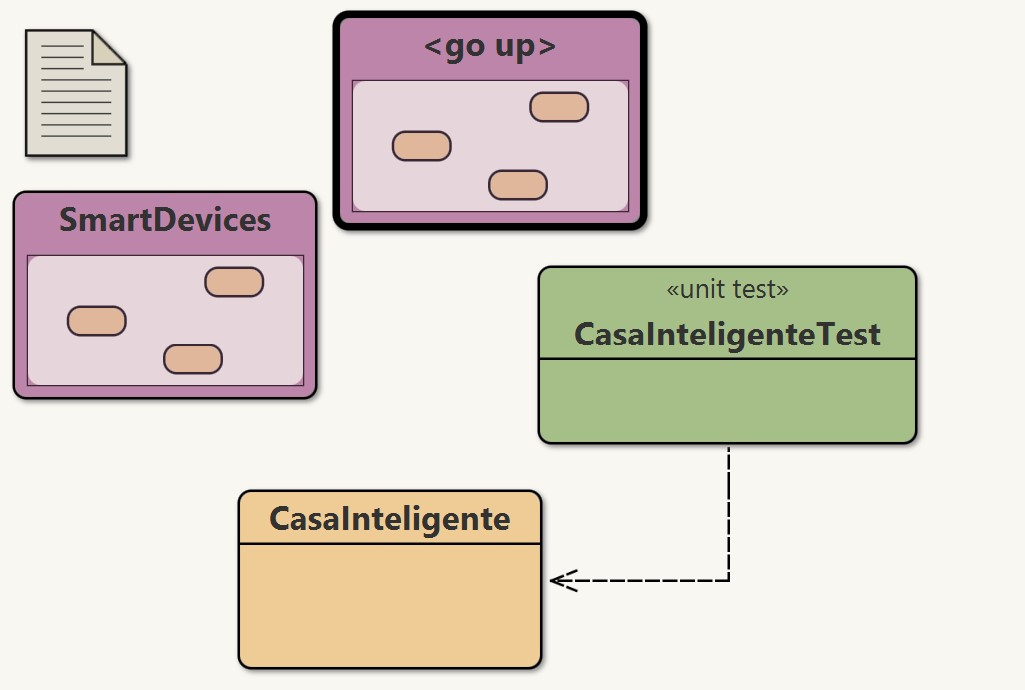
\includegraphics[scale=0.8]{diagrama2.jpg}
	\end{figure}
	
\item Diagrama da classe CasaInteligente
\vspace{15mm} %5mm vertical space

	\begin{figure}[H]
    		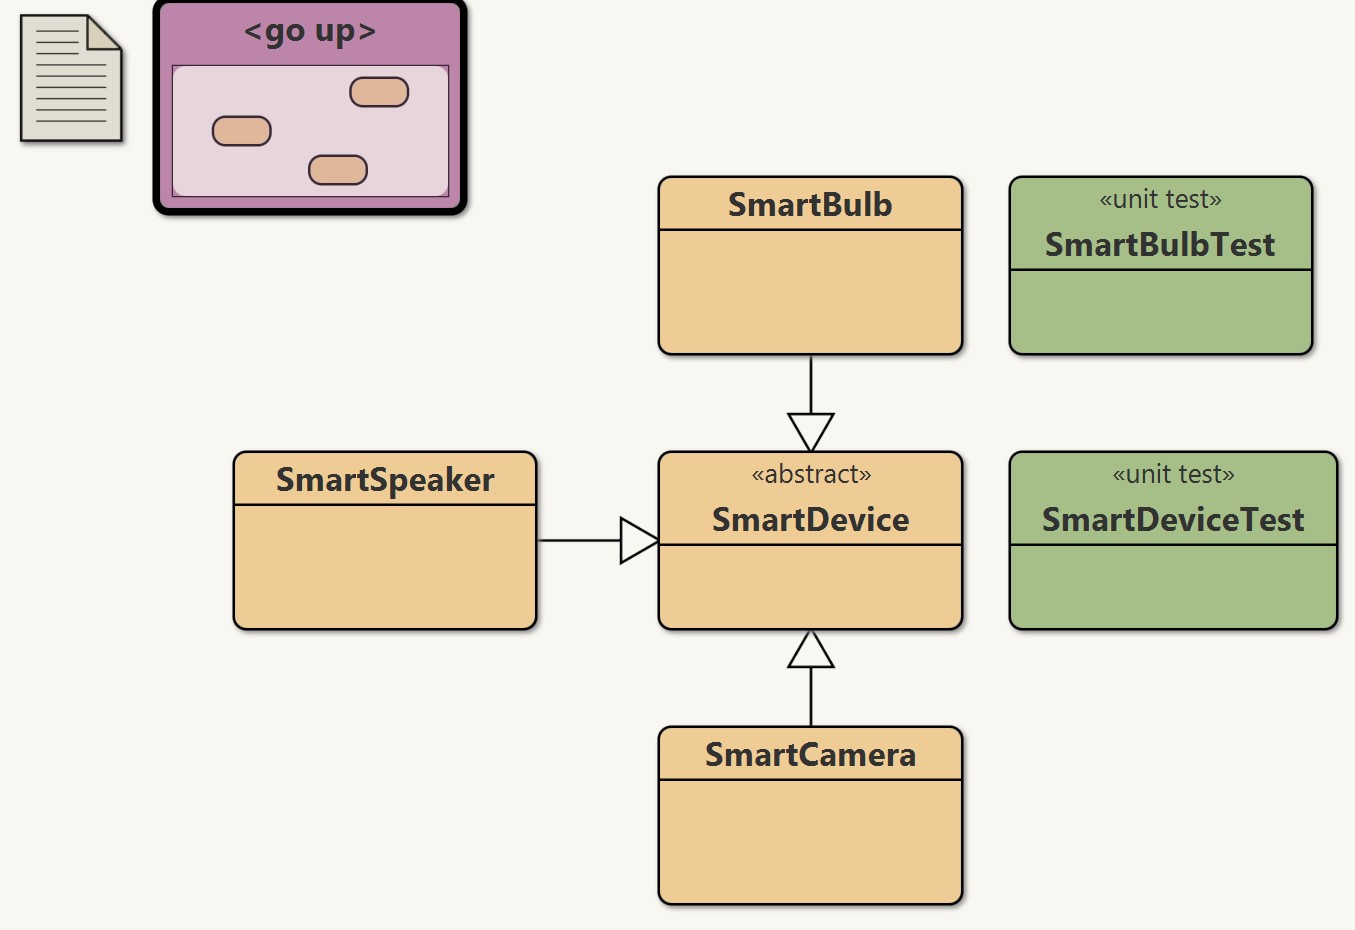
\includegraphics[scale=0.8]{diagrama3.jpg}
    \end{figure}
    
\item Diagrama da classe SmartDevices 
\vspace{15mm} %5mm vertical space

    \begin{figure}[H]
    		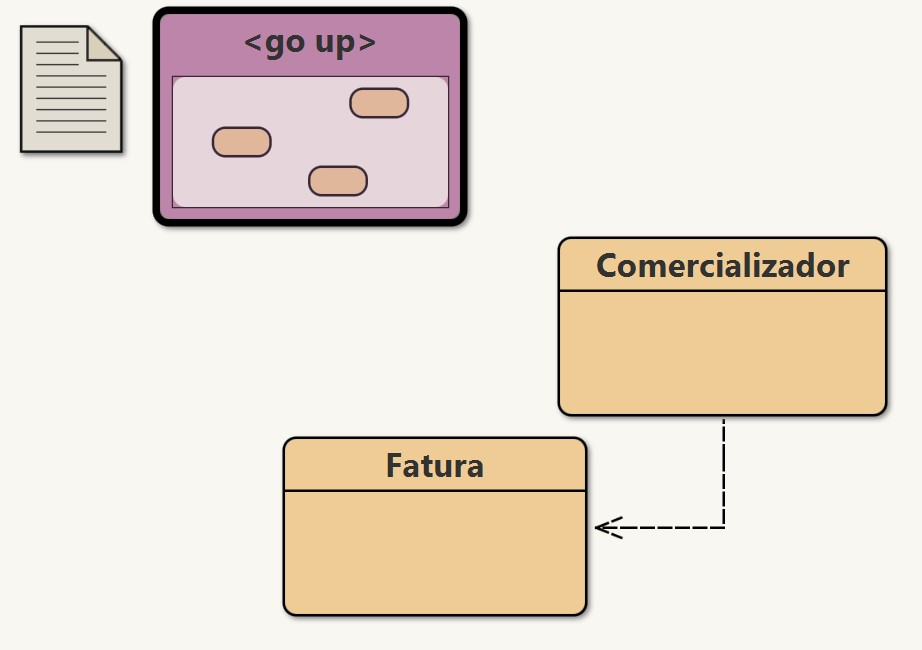
\includegraphics[scale=0.8]{diagrama4.jpg}
	\end{figure}
	
\item Diagrama da classe ComercializadoresEnergia

\end{enumerate}
    \pagebreak

\chapter{Diagrama do \textit{Intellij}}
    \begin{figure}[H]
        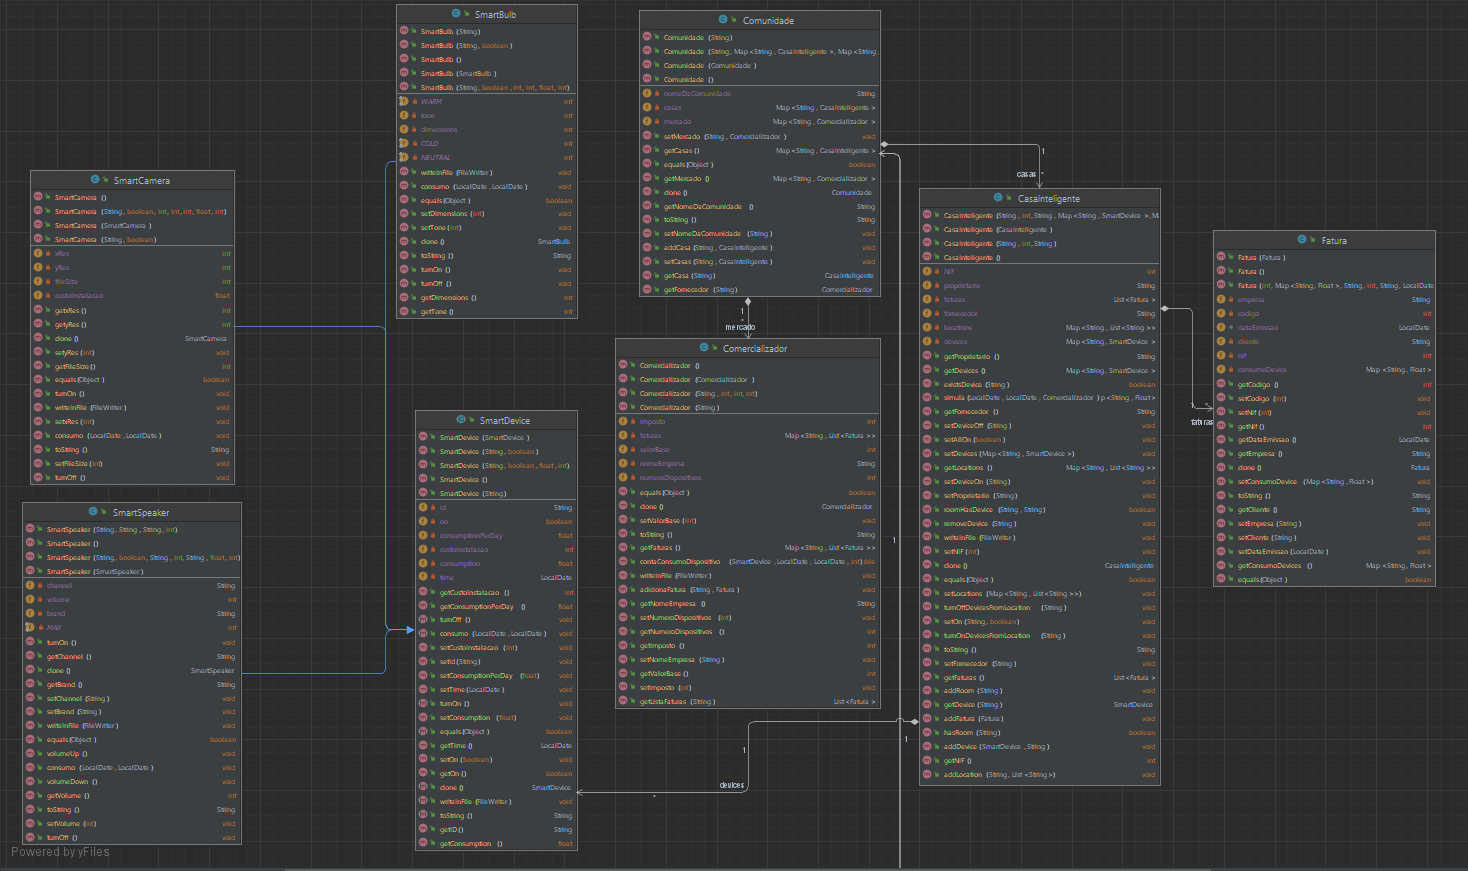
\includegraphics[scale=0.3]{diagrama itellij1.png}
	\end{figure}
	
	\begin{figure}[H]
        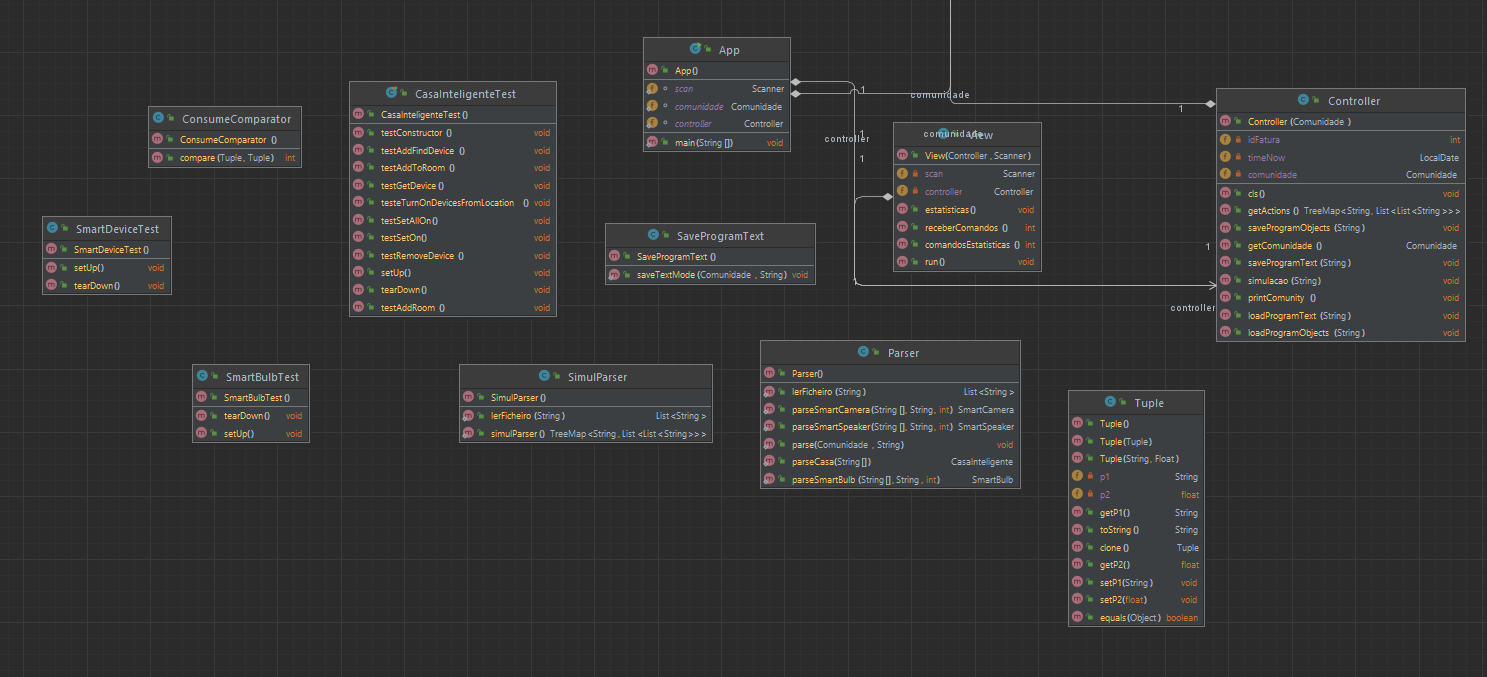
\includegraphics[scale=0.3]{diagrama intellij2.png}
	\end{figure}
	
	     
    
    
\pagebreak	
    \chapter{Funcionalidades do Programa}
    \section{Menu Principal}
    \begin{figure}[H]
        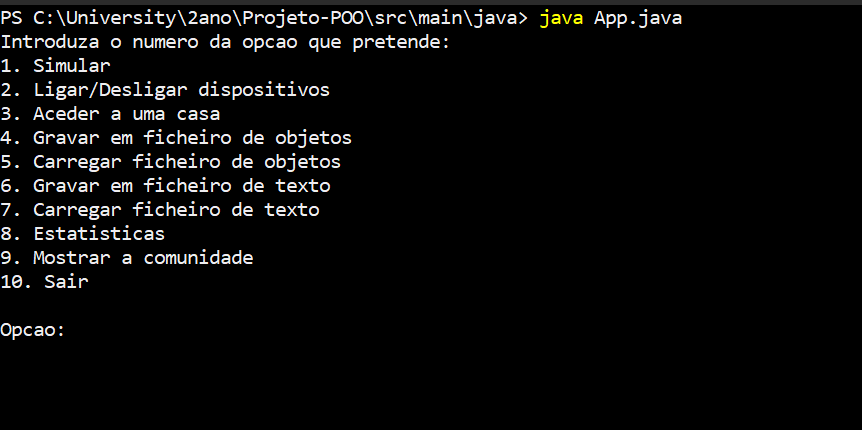
\includegraphics[scale=0.5]{menu1.png}
	\end{figure}
	
	\section{Menu Dispositivos}
	\begin{figure}[H]
        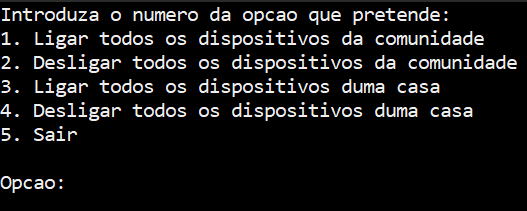
\includegraphics[scale=0.8]{menu2.png}
	\end{figure}
	
	\section{Menu Estatísticas}
	\begin{figure}[H]
        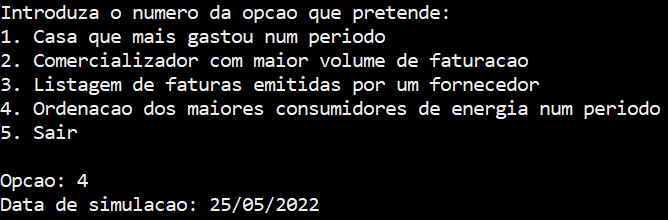
\includegraphics[scale=0.6]{menu3.png}
	\end{figure}
	

\pagebreak
	\chapter{Conclusão}
    
    Em conclusão, a nível geral, e tendo em conta o panorama apresentado nos capítulos anteriores e os objetivos pedidos para esta realização, como grupo, achamos que todos os objetivos foram cumpridos, conseguindo superar com sucesso, todas as dificuldades que fomos encontrando,  sempre com um olhar crítico e empenho. Acreditamos que aprendemos os conteúdos e objetivos desta Unidade Curricular e ,em particular, deste projeto.
	

\end{document}

